\documentclass{beamer}
\usepackage[italian]{babel}
\usepackage[autostyle, english = american]{csquotes}
\usepackage{graphicx}
\usepackage{parskip}
\usepackage{subcaption}
\usetheme{Boadilla}
\graphicspath{ {./} }
\begin{document}
\title{Esercitazione 4}
\subtitle{Esplorazione di sottocartelle e cancellazione di una parola da un file}
\author{Corradini, De Luca, di Nuzzo, Frick, Ragazzini}
\institute{unibo}
\date{2019}
\setbeamercovered{transparent}
\begin{frame}
\titlepage
\end{frame}
\begin{frame}{Eliminazione di parole - Servitore UDP}
Servitore sequenziale che permette la mutua esclusione sul file, ma per file molto lunghi ne risente anche il servizio TCP.

Definizione di "parola": \textbf{sequenza di caratteri} o stringhe separate da separatori? 
Scelta di progetto: stringhe separate.
\end{frame}

\begin{frame}{Esplorazione di direttori - Servitori TCP}
  Vengono esplorati solo i sottodirettori a partire dal secondo livello.

  È stata scelta una formattazione altamente leggibile.

  Il cliente riceve una sola stringa contenente l'intera risposta.

  Esempio di esecuzione: 

  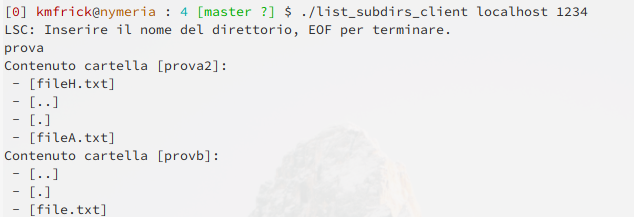
\includegraphics[width=\textwidth]{example}
\end{frame}
\begin{frame}{Conclusioni}
  Possibili ottimizzazioni:

  Il servizio UDP di cancellazione parole può essere ottimizzato generando un figlio per richiesta. 
  I figli però non devono agire in modo concorrente.

Il servizio TCP potrebbe non essere sicuro: permette di visualizzare anche cartelle di sistema. 
È richiesto un uso appropriato dei permessi del filesystem.
\end{frame}

\end{document}
